\chapter{Фермионы, матрицы Дирака и море Дирака}

Море Дирака — наша цель, но путь к нему тоже важен. Прежде чем столкнуться с отрицательной энергией в релятивистской теории электрона, нам понадобятся два элемента формализма. Сначала идет операторная алгебра, отличающая фермионы от бозонов. Затем — обзор одномерного уравнения Дирака, где любое расширение волновой функции можно проследить без геометрии трех пространственных измерений. Когда эти элементы будут на месте, трехмерное уравнение само потребует матричной структуры, а начальное обсуждение заполненных и пустых фермионных состояний вернется как ключ к позитронам.

Мы используем \(c=\hbar=1\). Заглавная \(P\) обозначает оператор импульса, строчная \(p\) — собственное значение импульса, а полужирные символы — их трехмерные версии.

\section{Обмен задается операторной алгеброй}

Рассмотрим две тождественные частицы, одну в \(x\) и другую в \(y\). Метки \(x\) и \(y\) обозначают полные положения; это не две декартовы координаты одной частицы. Действуя на вакуум двумя операторами рождения, получаем
\begin{equation}
\lvert x,y\rangle
=
\psi^\dagger(x)\psi^\dagger(y)\lvert0\rangle.
\label{eq:l10-two-particle-state}
\end{equation}

Для бозонов перестановка двух аргументов не меняет состояние:
\begin{equation}
\lvert x,y\rangle=\lvert y,x\rangle.
\end{equation}
Операторное утверждение, гарантирующее эту симметрию, имеет вид
\begin{equation}
\psi^\dagger(x)\psi^\dagger(y)
=
\psi^\dagger(y)\psi^\dagger(x).
\label{eq:l10-boson-exchange}
\end{equation}
Два бозонных оператора рождения коммутируют, поэтому мы можем менять их порядок, не изменяя создаваемое ими состояние.

Для фермионов перестановка меняет знак:
\begin{equation}
\lvert x,y\rangle=-\lvert y,x\rangle.
\label{eq:l10-fermion-state-exchange}
\end{equation}
Общий знак изолированного вектора состояния ненаблюдаем, но относительные знаки между альтернативами наблюдаемы, поэтому этот минус нужно последовательно сохранять. Из уравнения~\eqref{eq:l10-fermion-state-exchange} следует
\begin{equation}
\psi^\dagger(x)\psi^\dagger(y)
=
-\,\psi^\dagger(y)\psi^\dagger(x).
\label{eq:l10-fermion-operator-exchange}
\end{equation}

\begin{figure}[htbp]
\centering
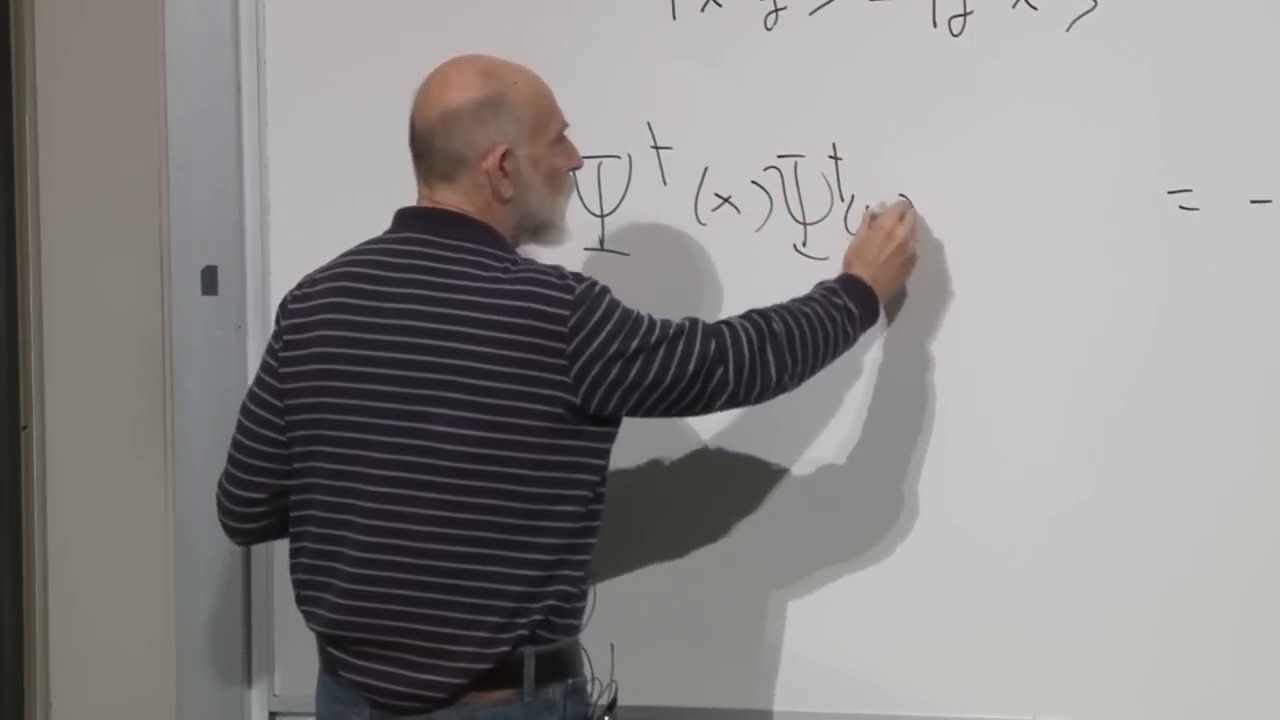
\includegraphics[width=0.94\linewidth]{lecture_10_figure_02.png}
\caption{Соотношение на доске, реализующее фермионный обмен. При перестановке операторов рождения знак двухчастичного состояния меняется на противоположный.}
\lectureframe{00:05:50}
\end{figure}

Для любых двух операторов \(A\) и \(B\) определим антикоммутатор как
\begin{equation}
\{A,B\}:=AB+BA.
\end{equation}
Поэтому правило обмена имеет вид
\begin{equation}
\{\psi^\dagger(x),\psi^\dagger(y)\}=0.
\label{eq:l10-creation-anticommutator}
\end{equation}
Соответствующая алгебра фермионного поля заменяет бозонные коммутаторы антикоммутаторами. Нужно различать два употребления этого термина: полевые операторы антикоммутируют в силу статистики Ферми, тогда как матрицы позднее будут антикоммутировать, чтобы устранить перекрестные члены в релятивистском дисперсионном соотношении.

Теперь положим \(y=x\) в уравнении~\eqref{eq:l10-creation-anticommutator}. Оба произведения становятся одинаковыми:
\begin{align}
0
&=\{\psi^\dagger(x),\psi^\dagger(x)\}\\
&=2\,\psi^\dagger(x)\psi^\dagger(x).
\end{align}
Следовательно,
\begin{equation}
\bigl(\psi^\dagger(x)\bigr)^2=0.
\label{eq:l10-exclusion}
\end{equation}
Попытка создать два тождественных фермиона в одном и том же одночастичном состоянии дает нулевой вектор. Это и есть принцип исключения в операторной форме.

\begin{figure}[htbp]
\centering
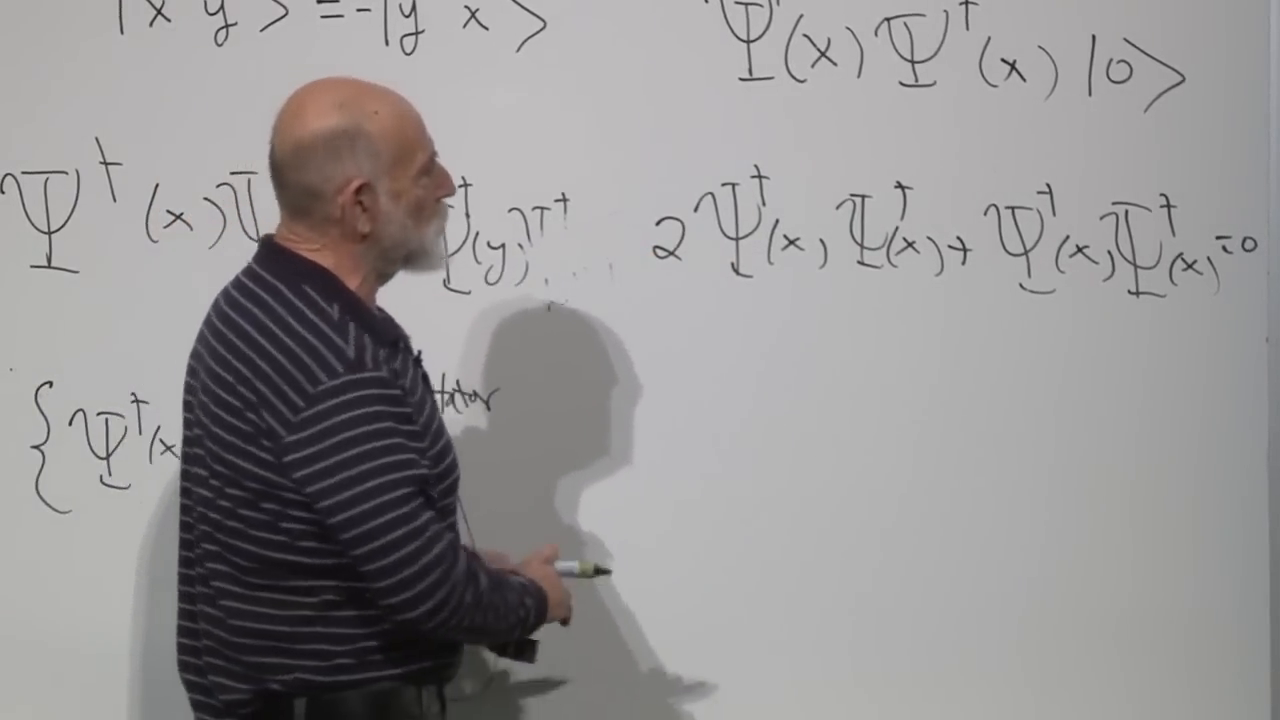
\includegraphics[width=0.94\linewidth]{lecture_10_figure_03.png}
\caption{Специализация на случай одинаковых состояний на доске. Произведение одного и того же оператора рождения появляется дважды и поэтому должно обращаться в нуль.}
\lectureframe{00:08:04}
\end{figure}

\begin{figure}[htbp]
\centering
\begin{adjustbox}{max width=\linewidth}
\begin{tikzpicture}[node distance=1.25cm,>=Latex]
\node[draw,rounded corners,align=center,inner sep=7pt] (a)
  {$\{\psi^\dagger(x),\psi^\dagger(x)\}=0$};
\node[draw,rounded corners,align=center,inner sep=7pt,right=of a] (b)
  {$2(\psi^\dagger(x))^2=0$};
\node[draw,rounded corners,align=center,inner sep=7pt,right=of b] (c)
  {$(\psi^\dagger(x))^2=0$};
\draw[->,thick] (a) -- (b);
\draw[->,thick] (b) -- (c);
\end{tikzpicture}
\end{adjustbox}
\caption{Вывод принципа исключения, восстановленный без частично стёртых промежуточных записей на доске.}
\end{figure}

\section{Почему заполненное и пустое симметричны для фермиона}

Есть и второе различие между бозонными и фермионными операторами, более тонкое, чем принцип исключения, и важное для дальнейшего. Для одной бозонной моды,
\begin{equation}
[a,a^\dagger]=1,
\qquad
n=0,1,2,\ldots.
\end{equation}
Перестановка \(a\) и \(a^\dagger\) меняет знак коммутатора. Даже если бы операторы просто назывались \(A\) и \(B\), алгебра сказала бы нам, какое упорядочение повышает число заполнения, а какое понижает его.

У бозонной лестницы заполнения тоже есть ориентация. Оператор уничтожения в конце концов доходит до \(\lvert0\rangle\) и дает нуль, тогда как оператор рождения может действовать неограниченно:
\begin{align}
a\lvert0\rangle&=0,\\
a^\dagger\lvert n\rangle&\propto\lvert n+1\rangle,
\qquad n=0,1,2,\ldots.
\end{align}
Если перевернуть эту лестницу вверх ногами, тот же спектр не получится. У нее есть низ, но нет верха.

Для одной фермионной моды,
\begin{equation}
\{a,a^\dagger\}=1,
\qquad
a^2=(a^\dagger)^2=0,
\qquad
n=0,1.
\label{eq:l10-fermion-mode}
\end{equation}
Оператор рождения переводит пустое состояние в заполненное, а затем останавливается:
\begin{equation}
a^\dagger\lvert0\rangle=\lvert1\rangle,
\qquad
a^\dagger\lvert1\rangle=0.
\end{equation}
Оператор уничтожения выполняет обратное:
\begin{equation}
a\lvert1\rangle=\lvert0\rangle,
\qquad
a\lvert0\rangle=0.
\end{equation}
Состояний только два, поэтому схема симметрична относительно замены заполненного на пустое и \(a\) на \(a^\dagger\). Физические смыслы операторов по-прежнему различны, но их алгебра уже не выделяет один как рождение, а другой как уничтожение. Эта формальная симметрия — зерно переинтерпретации частица–дырка.

\begin{classroomqa}
\lecturetimestamp{00:13:54}
\audiencequestion{Если \((a^\dagger)^2=0\), то это противоречие или отсюда следует, что \(a^\dagger=0\)?}
\lecturerresponse{Ни то ни другое. Ненулевой оператор может иметь обращающийся в нуль квадрат. Здесь \(a^\dagger\) переводит \(\lvert0\rangle\) в \(\lvert1\rangle\), но выше \(\lvert1\rangle\) допустимого состояния нет, поэтому двукратное применение дает нуль. То же рассуждение дает \(a^2=0\).}
\end{classroomqa}

Сохраним эту симметрию заполненного и пустого про запас. Когда электрон с отрицательной энергией удаляется, оператор уничтожения будет переобозначен как оператор рождения позитрона. Этот шаг — не произвольная смена обозначений; он использует в точности ту двухсостоянную фермионную алгебру, которая установлена здесь.

\section{Одномерная конструкция Дирака}

Теперь вернемся к одной частице в одном пространственном измерении. Простейшее релятивистское волновое уравнение первого порядка имеет вид
\begin{equation}
i\partial_t\psi=-\,i\partial_x\psi.
\label{eq:l10-right-mover}
\end{equation}
При \(P=-i\partial_x\) это
\begin{equation}
H=P.
\end{equation}
Для собственного состояния импульса имеем \(E=p\), а его групповая скорость равна
\begin{equation}
v_g=\frac{dE}{dp}=1.
\end{equation}
Положительный или отрицательный импульс, а значит, и положительная или отрицательная энергия, все равно дает волну, движущуюся вправо без изменения формы. Знак \(p\) меняет фазовый рисунок, а не направление распространения.

Массивная частица должна иметь возможность двигаться в любом направлении. Введем вторую компоненту, удовлетворяющую
\begin{equation}
H\psi_1=P\psi_1,
\qquad
H\psi_2=-P\psi_2.
\label{eq:l10-two-directions}
\end{equation}
Первая компонента движется вправо, вторая — влево. Объединим их в столбец,
\begin{equation}
\Psi=
\begin{pmatrix}
\psi_1\\
\psi_2
\end{pmatrix},
\end{equation}
и определим
\begin{equation}
\alpha=
\begin{pmatrix}
1&0\\
0&-1
\end{pmatrix}.
\end{equation}
Тогда оба уравнения принимают вид
\begin{equation}
H\Psi=\alpha P\Psi.
\label{eq:l10-massless-one-d}
\end{equation}
Цена включения обоих направлений — новая внутренняя степень свободы с двумя значениями.

Само по себе направление не порождает массу. Введем вторую матрицу,
\begin{equation}
\beta=
\begin{pmatrix}
0&1\\
1&0
\end{pmatrix},
\end{equation}
и попробуем
\begin{equation}
H=\alpha P+\beta m.
\label{eq:l10-massive-one-d}
\end{equation}
Эти матрицы удовлетворяют соотношениям
\begin{equation}
\alpha^2=\beta^2=\mathbb{1},
\qquad
\{\alpha,\beta\}=0.
\label{eq:l10-one-d-algebra}
\end{equation}
Возведение гамильтониана в квадрат дает
\begin{align}
H^2
&=(\alpha P+\beta m)^2\\
&=\alpha^2P^2+\beta^2m^2
  +(\alpha\beta+\beta\alpha)Pm\\
&=P^2+m^2.
\label{eq:l10-one-d-dispersion}
\end{align}
Антикоммутатор в уравнении~\eqref{eq:l10-one-d-algebra} устраняет нежелательный член, линейный и по \(P\), и по \(m\).

Недиагональная матрица \(\beta\) связывает две направленные компоненты. Полезно представлять массовый член как непрерывно смешивающий амплитуды, движущиеся вправо и влево. Эту картину не следует понимать буквально как частицу, отскакивающую туда-сюда по микроскопической траектории, но она передает, почему массивный волновой пакет может иметь среднюю скорость меньше скорости света и собственную систему отсчета, тогда как изолированная безмассовая хиральная компонента — нет.

\begin{classroomqa}
\lecturetimestamp{00:23:37}
\audiencequestion{Есть ли более глубокая физическая интерпретация введения обеих направленных компонент?}
\lecturerresponse{Есть, но яснее она проявится в трех измерениях. На этом этапе это просто две компоненты, необходимые для описания противоположных направлений распространения и для того, чтобы допустить недиагональную массовую связь. Их более поздняя интерпретация — лево- и праворукость, то есть хиральность.}
\end{classroomqa}

\section{Три измерения требуют матриц Паули}

В трех пространственных измерениях импульс является вектором. Поэтому гамильтониан, линейный по импульсу и скалярный относительно вращений, подсказывает другой вектор — теперь вектор, компонентами которого являются матрицы:
\begin{equation}
H=\boldsymbol{\alpha}\cdot\mathbf P
=\alpha_xP_x+\alpha_yP_y+\alpha_zP_z.
\label{eq:l10-three-d-ansatz}
\end{equation}

\begin{figure}[htbp]
\centering
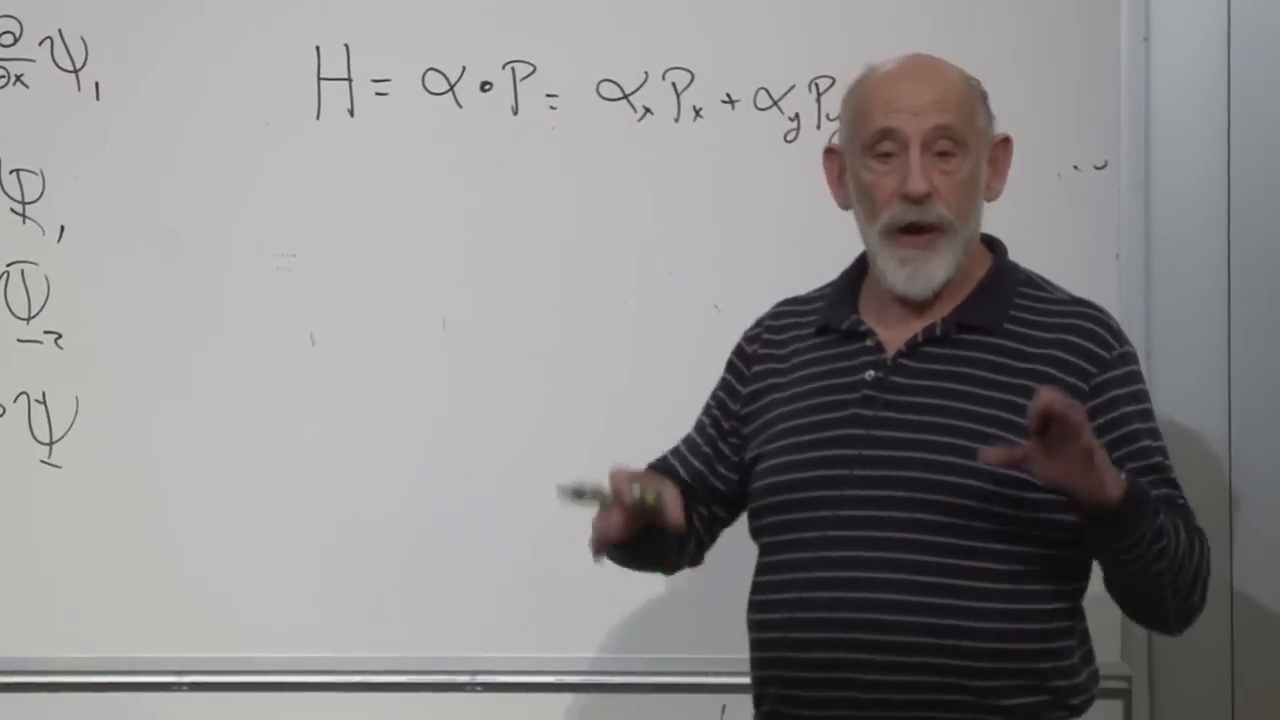
\includegraphics[width=0.94\linewidth]{lecture_10_figure_04.png}
\caption{Трехмерный безмассовый анзац \(H=\boldsymbol{\alpha}\cdot\mathbf P\) в тот момент, когда одна матрица становится вектором из трех матриц.}
\lectureframe{00:26:00}
\end{figure}

Снова начнем с безмассового случая. Мы требуем, чтобы
\begin{equation}
H^2=\mathbf P^2=P_x^2+P_y^2+P_z^2.
\end{equation}
Раскрывая квадрат уравнения~\eqref{eq:l10-three-d-ansatz},
\begin{align}
H^2
&=\alpha_x^2P_x^2+\alpha_y^2P_y^2\\
&\quad+\alpha_z^2P_z^2\\
&\quad+\{\alpha_x,\alpha_y\}P_xP_y\\
&\quad+\{\alpha_x,\alpha_z\}P_xP_z\\
&\quad+\{\alpha_y,\alpha_z\}P_yP_z.
\end{align}
Диагональные члены правильны, если
\begin{equation}
\alpha_x^2=\alpha_y^2=\alpha_z^2=\mathbb{1},
\end{equation}
а все перекрестные члены исчезают, если
\begin{equation}
\{\alpha_i,\alpha_j\}=0,
\qquad i\ne j.
\label{eq:l10-alpha-anticommutation}
\end{equation}

Три знакомые матрицы \(2\times2\) делают ровно это:
\begin{equation}
\sigma_x=
\begin{pmatrix}
0&1\\
1&0
\end{pmatrix},
\quad
\sigma_y=
\begin{pmatrix}
0&-i\\
i&0
\end{pmatrix},
\quad
\sigma_z=
\begin{pmatrix}
1&0\\
0&-1
\end{pmatrix}.
\label{eq:l10-pauli-matrices}
\end{equation}
Таким образом, одним из решений является
\begin{equation}
\alpha_i=\sigma_i,
\qquad
H=\boldsymbol{\sigma}\cdot\mathbf P.
\label{eq:l10-weyl-hamiltonian}
\end{equation}

\begin{figure}[htbp]
\centering
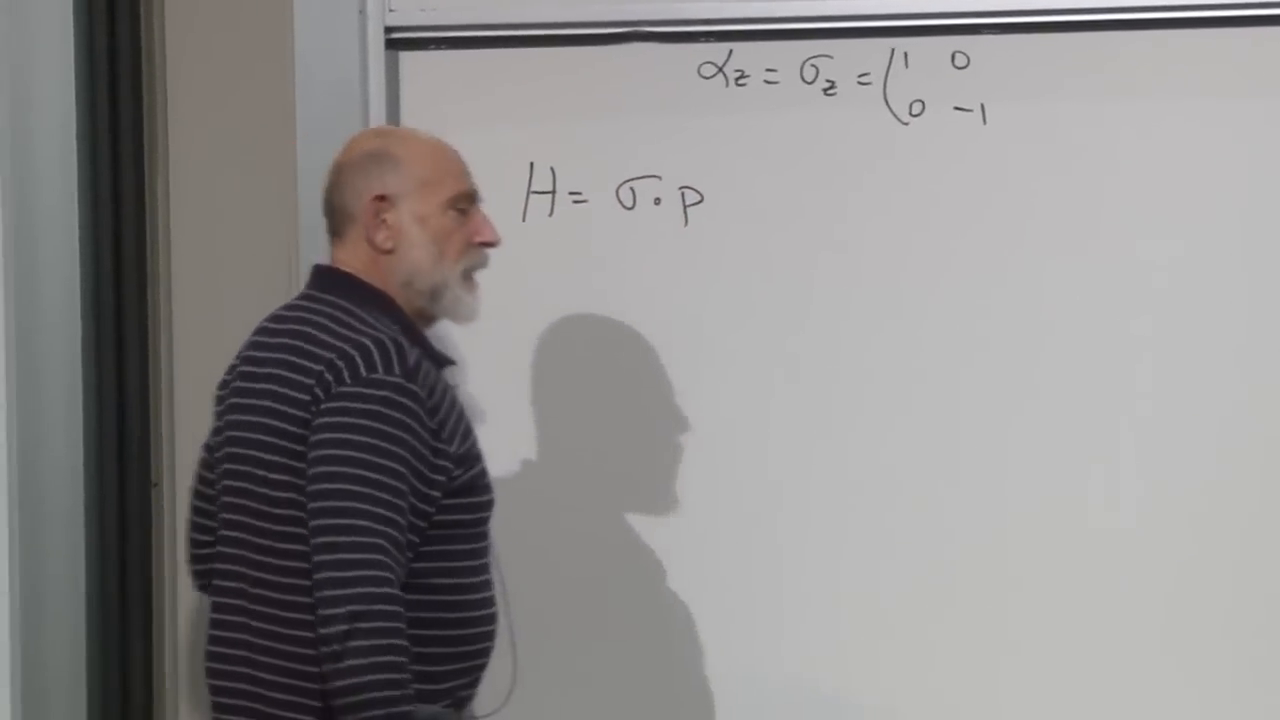
\includegraphics[width=0.94\linewidth]{lecture_10_figure_05.png}
\caption{Компактный безмассовый гамильтониан \(H=\boldsymbol{\sigma}\cdot\mathbf P\); над ним по-прежнему видна запись \(\alpha_z=\sigma_z\).}
\lectureframe{00:28:16}
\end{figure}

Для собственного состояния импульса,
\begin{equation}
\boldsymbol{\sigma}\cdot\mathbf p
=
|\mathbf p|\,\boldsymbol{\sigma}\cdot\widehat{\mathbf p}.
\end{equation}
Оператор \(\boldsymbol{\sigma}\cdot\widehat{\mathbf p}\) имеет собственные значения \(+1\) и \(-1\), так что
\begin{equation}
E=\pm|\mathbf p|.
\end{equation}
В этой двухкомпонентной теории положительной энергии соответствует степень свободы Паули, сонаправленная с импульсом, а отрицательной — направленная противоположно ему. Эта сонаправленность фиксирована; это не независимо выбираемое направление спина при фиксированном знаке энергии.

\begin{classroomqa}
\lecturetimestamp{00:30:10}
\audiencequestion{Спин «выпадает» из уравнения Дирака, или он был внесен потому, что уже известно, что у электрона есть магнитный момент?}
\lecturerresponse{Здесь «выпадает» означает «появляется как следствие», а не «исчезает». Исходным требованием был гамильтониан, линейный по импульсу, квадрат которого равен \(\mathbf P^2\). Обычные числа не могут удовлетворить требуемым алгебраическим соотношениям, а матрицы Паули могут. Поэтому их двухкомпонентная структура появляется вместе с самой линеаризацией. Это не доказывает, что каждая частица обязана иметь спин; это говорит о том, что частицы, описываемые уравнением дираковского типа, несут соответствующую спинорную степень свободы.}
\end{classroomqa}

Это один из центральных уроков данного построения. Матрицы — не декоративные метки, добавляемые после того, как найдено релятивистское уравнение. Их порождает попытка локально извлечь квадратный корень из релятивистского дисперсионного соотношения.

\section{Почему для массы нужны четыре компонента}

Попробуем повторить одномерное построение массы, не расширяя теорию \(2\times2\):
\begin{equation}
H=\boldsymbol{\sigma}\cdot\mathbf P+\beta m.
\label{eq:l10-failed-mass}
\end{equation}
Предположим, что \(\beta^2=\mathbb{1}\). Квадрат содержит требуемые члены \(\mathbf P^2+m^2\), но также содержит
\begin{equation}
m\sum_i\{\sigma_i,\beta\}P_i.
\end{equation}
Чтобы устранить этот член, матрица \(\beta\) должна была бы удовлетворять
\begin{equation}
\{\sigma_x,\beta\}
=
\{\sigma_y,\beta\}
=
\{\sigma_z,\beta\}
=0.
\label{eq:l10-impossible-beta}
\end{equation}
Ни одна матрица \(2\times2\) этому не удовлетворяет. Единичная матрица коммутирует со всеми тремя матрицами Паули, а всякая бесследовая матрица \(2\times2\) является линейной комбинацией матриц Паули. Любая такая комбинация не антикоммутирует с компонентой, параллельной ей. В алгебре \(2\times2\) нет четвёртой независимой матрицы требуемого вида.

Выход состоит в том, чтобы увеличить спинор. Четыре попарно антикоммутирующие матрицы, квадраты которых равны единичной матрице, впервые появляются в комплексном представлении \(4\times4\). Этот размер матриц выбирается не потому, что пространство-время четырёхмерно; это наименьшее матричное пространство, способное реализовать требуемую алгебру.

Существует много эквивалентных представлений. Унитарная замена спинорного базиса изменяет элементы всех матриц, не меняя ни одного физического предсказания. Существен лишь абстрактный набор соотношений
\begin{equation}
\{\alpha_i,\alpha_j\}=2\delta_{ij}\mathbb{1},
\qquad
\{\alpha_i,\beta\}=0,
\qquad
\beta^2=\mathbb{1}.
\label{eq:l10-dirac-algebra}
\end{equation}

\begin{classroomqa}
\lecturetimestamp{00:37:38}
\audiencequestion{Можно ли рассматривать \(\beta\) как временную компоненту \(\alpha_t\)?}
\lecturerresponse{Не напрямую. Три \(\alpha_i\) не образуют вместе с \(\beta\) четыре компоненты одного лоренцева вектора. В ковариантной записи вместо этого определяют \(\beta=\gamma^0\) и \(\alpha_i=\gamma^0\gamma^i\); четыре матрицы \(\gamma^\mu\) удовлетворяют пространственно-временной алгебре Клиффорда.}
\end{classroomqa}

Удобное блочное представление имеет вид
\begin{equation}
\alpha_i=
\begin{pmatrix}
\sigma_i&0\\
0&-\sigma_i
\end{pmatrix},
\qquad
\beta=
\begin{pmatrix}
0&I_2\\
I_2&0
\end{pmatrix}.
\label{eq:l10-block-representation}
\end{equation}
Матрицы Паули в диагональных блоках гарантируют, что различные \(\alpha_i\) антикоммутируют. Внедиагональные единичные блоки в \(\beta\) гарантируют, что \(\beta\) антикоммутирует с каждым \(\alpha_i\).

\begin{figure}[htbp]
\centering
\includegraphics[width=0.94\linewidth]{lecture_10_figure_06.png}
\caption{Блочное представление \(4\times4\), выписанное на доске. Верхние уравнения задают требуемые антикоммутаторы; полные матрицы набраны в уравнении~\eqref{eq:l10-block-representation}.}
\lectureframe{00:41:10}
\end{figure}

Массивный гамильтониан теперь имеет вид
\begin{equation}
H=\boldsymbol{\alpha}\cdot\mathbf P+\beta m
=
\begin{pmatrix}
\boldsymbol{\sigma}\cdot\mathbf P&mI_2\\
mI_2&-\boldsymbol{\sigma}\cdot\mathbf P
\end{pmatrix}.
\label{eq:l10-massive-dirac}
\end{equation}
Используя уравнение~\eqref{eq:l10-dirac-algebra},
\begin{equation}
H^2=\mathbf P^2+m^2.
\end{equation}
Следовательно, четырёхкомпонентная структура — не необязательное украшение. Это наименьшая структура, допускающая и трёхмерный импульс, и массовый член при сохранении уравнения первого порядка.

\section{Хиральность и смысл дополнительных компонент}

Какое физическое различие добавило это расширение? Начнём с безмассового верхнего блока,
\begin{equation}
H_R=\boldsymbol{\sigma}\cdot\mathbf P,
\end{equation}
и безмассового нижнего блока,
\begin{equation}
H_L=-\boldsymbol{\sigma}\cdot\mathbf P.
\end{equation}
Для состояний с положительной энергией у первого спин сонаправлен с импульсом, а у второго — антинаправлен. Это противоположные спиральности. В безмассовой теории спиральность инвариантна относительно собственных преобразований Лоренца, потому что ни один наблюдатель не может обогнать светоподобную частицу и обратить её импульс, оставив её спин неизменным. Поэтому два блока описывают противоположные хиральные секторы.

\begin{classroomqa}
\lecturetimestamp{00:41:28}
\audiencequestion{В одном измерении для введения массы требовалась дополнительная двоичная степень свободы. Какому физическому различию она соответствует в трёх измерениях?}
\lecturerresponse{Это хиральность спинора. Два блока \(2\times2\) задают противоположные соотношения между спином и импульсом. Один правохирален, другой левохирален. Теория \(4\times4\) содержит оба.}
\end{classroomqa}

Массовый член в уравнении~\eqref{eq:l10-massive-dirac} внедиагонален. Он переводит амплитуду верхнего блока в нижний и наоборот:
\begin{equation}
\beta m
\begin{pmatrix}
\Psi_R\\
\Psi_L
\end{pmatrix}
=
m
\begin{pmatrix}
\Psi_L\\
\Psi_R
\end{pmatrix}.
\end{equation}
Следовательно, масса представляет собой связь между противоположными хиральностями.

\begin{classroomqa}
\lecturetimestamp{00:43:58}
\audiencequestion{Может ли безмассовая частица изменить хиральность?}
\lecturerresponse{Не в свободном безмассовом гамильтониане, выписанном здесь. Два блока развязаны, так что состояние, начавшееся как правохиральное или левохиральное, таким и остаётся. Именно внедиагональный массовый член смешивает их при \(m\ne0\).}
\end{classroomqa}

Этот язык точен для блочного представления, но картину частицы, механически перескакивающей между двумя стрелками, не следует понимать слишком буквально. Физическое содержание состоит в матричной связи в волновом уравнении.

\begin{classroomqa}
\lecturetimestamp{00:44:50}
\audiencequestion{Содержатся ли эти матрицы уже в кватернионах?}
\lecturerresponse{Матрицы Паули тесно связаны с кватернионными единицами: матрицы \(-i\sigma_i\) возводятся в \(-\mathbb{1}\) и перемножаются по кватернионному правилу с точностью до соглашений об ориентации. Полные матрицы Дирака требуют большей алгебры Клиффорда, и для следующего рассуждения связь с кватернионами не нужна.}
\end{classroomqa}

\begin{classroomqa}
\lecturetimestamp{00:46:34}
\audiencequestion{Если спин — это момент импульса, есть ли здесь отдельный энергетический член, связанный с ним?}
\lecturerresponse{Нет, никакого независимого члена для свободной частицы не добавляется. Спинорная структура уже входит в кинетический гамильтониан через матрицы. Связь спина с внешним магнитным полем ввела бы дополнительные члены взаимодействия, но это другая задача.}
\end{classroomqa}

\section{Матрицы альфа — это скорость, а не спин}

У каждой \(\alpha_i\) есть два собственных значения \(+1\) и два собственных значения \(-1\). Различные компоненты не коммутируют, поэтому их нельзя все одновременно измерить точно. Чтобы определить, что представляет собой одна из компонент, воспользуемся уравнением Гейзенберга. Для оператора \(L\) без явной зависимости от времени,
\begin{equation}
\dot L=i[H,L].
\label{eq:l10-heisenberg}
\end{equation}
Здесь соглашение о знаке фиксируется эволюцией Schr\"odinger \(e^{-iHt}\).

Применим уравнение~\eqref{eq:l10-heisenberg} к оператору положения \(x\). Матрицы действуют на спинорные индексы и коммутируют с положением, тогда как только \(P_x\) не коммутирует с \(x\):
\begin{align}
\dot x
&=i[\boldsymbol{\alpha}\cdot\mathbf P+\beta m,x]\\
&=i\alpha_x[P_x,x]\\
&=\alpha_x,
\label{eq:l10-velocity}
\end{align}
поскольку \([P_x,x]=-i\). Следовательно, \(\alpha_x\) — это \(x\)-компонента оператора скорости; аналогично,
\begin{equation}
\dot{\mathbf x}=\boldsymbol{\alpha}.
\end{equation}

\begin{classroomqa}
\lecturetimestamp{00:51:50}
\audiencequestion{Неужели измерение компоненты скорости действительно даёт только \(+1\) или \(-1\)?}
\lecturerresponse{Да, для мгновенного оператора \(\alpha_i\) в единицах \(c=1\). Общее состояние не обязано быть собственным состоянием, поэтому его среднее значение может лежать где угодно между этими значениями. У гладко распространяющегося волнового пакета средняя скорость меньше световой, когда частица массивна.}
\end{classroomqa}

Скорость не сохраняется:
\begin{equation}
\dot\alpha_x=i[H,\alpha_x]\ne0.
\end{equation}
Слагаемые, содержащие \(\alpha_y\), \(\alpha_z\) и \(\beta\), не коммутируют с \(\alpha_x\). Поэтому состояние, содержащее компоненты как с положительной, так и с отрицательной энергией, даёт быстро осциллирующий вклад в положение. Это \emph{zitterbewegung}, буквально — дрожащее движение.

После усреднения по временам, большим по сравнению с быстрыми осцилляциями, ожидаемая релятивистская скорость равна
\begin{equation}
\overline{\mathbf v}=\frac{\mathbf p}{E},
\end{equation}
что для медленного электрона сводится к \(\mathbf p/m\).

\begin{classroomqa}
\lecturetimestamp{00:54:40}
\audiencequestion{Нарушает ли свободный электрон, дрожащий без внешней силы, закон Ньютона?}
\lecturerresponse{Нет. Трансляционная инвариантность сохраняет импульс, так что \(\dot{\mathbf P}=0\). Оператор скорости Дирака — не просто \(\mathbf P/m\), и его быстро осциллирующая часть может изменяться, тогда как импульс остаётся фиксированным. Усреднённое по времени движение подчиняется ожидаемому соотношению для свободной частицы.}
\end{classroomqa}

\begin{classroomqa}
\lecturetimestamp{00:55:22}
\audiencequestion{Всегда ли скорость равна \(c\)?}
\lecturerresponse{Мгновенное измерение одного \(\alpha_i\) имеет собственные значения \(\pm c\), но массивный волновой пакет, вообще говоря, является суперпозицией и имеет среднее значение меньше скорости света. Его средняя групповая скорость равна \(\mathbf p/E\).}
\end{classroomqa}

\begin{classroomqa}
\lecturetimestamp{00:55:30}
\audiencequestion{Можно ли понимать эти осцилляции так, будто масса изменяет скорость?}
\lecturerresponse{Нет. Масса — фиксированный параметр. Осцилляции возникают из-за некоммутирующих операторов скорости и гамильтониана, или, что эквивалентно, из-за интерференции между энергетическими секторами, а не из-за флуктуирующей массы.}
\end{classroomqa}

\begin{classroomqa}
\lecturetimestamp{00:56:22}
\audiencequestion{Может ли мгновенное измерение обнаружить скорость, направленную в одну сторону, даже если среднее движение направлено в другую?}
\lecturerresponse{Да. Оператор компоненты имеет два точных собственных значения, тогда как повторные или усреднённые по времени измерения восстанавливают более плавный дрейф.}
\end{classroomqa}

Слово спин тоже нужно употреблять осторожно. \(\alpha_i\) преобразуются как компоненты скорости, то есть обычного вектора. Подлинный оператор спина в этом представлении имеет вид
\begin{equation}
\mathbf S=\frac12\boldsymbol{\Sigma},
\qquad
\Sigma_i=
\begin{pmatrix}
\sigma_i&0\\
0&\sigma_i
\end{pmatrix}.
\label{eq:l10-spin-operator}
\end{equation}
Он отличается от \(\alpha_i\) знаком нижнего блока. Эти матрицы тесно связаны, но скорость и спин — не одна и та же наблюдаемая величина.

\section{Отрицательная энергия и вакуум с наименьшей энергией}

Проблема отрицательной энергии возникает уже до всего этого матричного аппарата. Вернёмся к одномерному праводвижущемуся состоянию,
\begin{equation}
H=P.
\end{equation}
Поскольку \(p\) пробегает всю вещественную ось, у \(E=p\) нет нижней границы.

Вакуум не может означать просто состояние без частиц. Он должен быть состоянием, из которого уже нельзя извлечь никакой дополнительной энергии. Если пустое состояние позволяет нам добавить частицу с отрицательной энергией, понизить энергию, добавить ещё одну и продолжать так бесконечно, то такое пустое состояние не является стабильным вакуумом.

Статистика Ферми исторически даёт выход. Поместим по одному электрону в каждое состояние с отрицательной энергией. Каждый добавленный электрон понижает полную энергию, но принцип запрета допускает только один электрон в каждом одночастичном состоянии. Когда все состояния с отрицательной энергией заполнены, никакой дополнительный электрон уже не может упасть в этот сектор. Дирак отождествил эту заполненную конфигурацию с вакуумом.

Та же конструкция не сработала бы для бозонов. Сколь угодно много бозонов может занимать одно состояние, так что бозонная мода с отрицательной энергией могла бы без ограничений поглощать частицы. Именно фермионное ограничение \(n=0,1\), введённое в начале лекции, и останавливает этот спуск.

\begin{figure}[htbp]
\centering
\includegraphics[width=0.94\linewidth]{lecture_10_figure_07.png}
\caption{Историческая картина моря Дирака на доске: лестница уровней отрицательной энергии, заполненных до разделяющей линии, а выше — состояния с положительной энергией.}
\lectureframe{01:02:45}
\end{figure}

\begin{figure}[htbp]
\centering
\begin{adjustbox}{max width=\linewidth}
\begin{tikzpicture}[x=1.05cm,y=0.72cm,>=Latex]
\draw[->] (0,-4.8) -- (0,4.8) node[above] {$E$};
\draw[thick] (-2.9,0) -- (3.2,0) node[right] {$E=0$};
\foreach \y in {-4,-3.3,...,-0.5} {
  \draw (-2.3,\y) -- (2.3,\y);
  \foreach \x in {-1.8,-1.2,...,1.8} {
    \fill[blue!65!black] (\x,\y) circle (1.6pt);
  }
}
\foreach \y in {0.8,1.6,...,4.0} {
  \draw (-2.3,\y) -- (2.3,\y);
}
\draw[red,very thick] (0.6,-2.6) circle (5pt);
\draw[red,->,very thick] (0.6,-2.35) .. controls (1.4,-0.4) and (1.2,1.6) .. (1.5,2.4);
\fill[red] (1.5,2.4) circle (2.5pt);
\node[right,red] at (0.85,-2.6) {hole};
\node[right,red] at (1.7,2.4) {$e^-$};
\node[left] at (-2.5,-2.2) {filled negative-energy states};
\end{tikzpicture}
\end{adjustbox}
\caption{Наглядная реконструкция возбуждения над заполненным морем: перевод одного электрона с отрицательной энергией оставляет дырку с положительной энергией.}
\end{figure}

Картина моря — это исторический язык для корректного переупорядочения операторов. Её буквальные бесконечные заряд и энергия не следует принимать за непосредственно наблюдаемые величины; современная переформулировка устранит необходимость представлять себе материальные электроны, заполняющие пространство.

\section{Дырка — это позитрон}

Когда все состояния с отрицательной энергией заняты, возможны два вида возбуждений. Можно добавить электрон с положительной энергией над морем. Или можно удалить один электрон с отрицательной энергией и оставить дырку.

Дырка имеет заряд, противоположный заряду отсутствующего электрона. Удаление заряда \(-e\) изменяет заряд на \(+e\). Она также имеет положительную энергию возбуждения. Если удалённый электрон имел \(E_-<0\), то энергия, измеренная относительно заполненного вакуума, изменяется на
\begin{equation}
E_{\mathrm{hole}}=-E_->0.
\end{equation}
Следовательно, дырка представляет собой возбуждение с положительной энергией и положительным зарядом: позитрон.

Фотон может перевести электрон из моря в состояние с положительной энергией. Относительно вакуума конечное состояние содержит электрон и позитрон. На диаграмме с временным упорядочением принято изображать поток электронного числа для электрона направленным вверх, а линию позитрона — со стрелкой в противоположную сторону. Эти стрелки отслеживают поток фермионного числа или заряда; это не маленькие классические векторы скорости.

\begin{classroomqa}
\lecturetimestamp{01:05:14}
\audiencequestion{Требует ли эта картина одинакового числа электронов и позитронов?}
\lecturerresponse{Не для произвольного состояния. Если начать с вакуума и создать нейтральную пару, получится по одному того и другого, но состояние уже может содержать избыток электронов или избыток позитронов. Сохранение заряда накладывает ограничения на реакции; оно не требует, чтобы в каждом допустимом состоянии их числа были равны.}
\end{classroomqa}

Дирак поначалу не знал, что дырка окажется частицей, тождественной электрону по массе и противоположной ему лишь по заряду и другим аддитивным квантовым числам. Уравнение и конструкция дырки привели к этому предсказанию ещё до того, как позитрон был включён в привычный каталог частиц.

\section{Одно фермионное поле содержит электроны и позитроны}

Оператор поля переводит историческую картину на язык современной алгебры. Пока опустим спинорные индексы, нормировочные множители и временную зависимость. Одномерное поле можно схематически разложить в виде
\begin{equation}
\psi(x)
\sim
\int_{-\infty}^{\infty}dp\,a(p)e^{ipx}.
\label{eq:l10-full-field-integral}
\end{equation}
Для праводвижущейся дисперсии \(E=p\) положительные значения \(p\) соответствуют положительной энергии, а отрицательные значения \(p\) — отрицательной. Разобьём интеграл:
\begin{equation}
\psi(x)
\sim
\int_0^\infty dp\,a(p)e^{ipx}
+
\int_{-\infty}^0 dp\,a(p)e^{ipx}.
\end{equation}
Во втором слагаемом положим \(p=-q\), где \(q>0\), и переинтерпретируем уничтожение заполненного электрона с отрицательной энергией как рождение позитрона:
\begin{equation}
b^\dagger(q):=a(-q).
\end{equation}
Тогда
\begin{equation}
\psi(x)
\sim
\int_0^\infty dp\,
\left[
a(p)e^{ipx}
+
b^\dagger(p)e^{-ipx}
\right].
\label{eq:l10-electron-positron-split}
\end{equation}
Точные знаки фаз плоских волн зависят от соглашения о пространстве-времени; инвариантное содержание состоит в том, что \(\psi\) содержит оператор уничтожения электрона и оператор рождения позитрона.

\begin{figure}[htbp]
\centering
\includegraphics[width=0.94\linewidth]{lecture_10_figure_08.png}
\caption{Интеграл по полю разделён на секторы положительной и отрицательной энергии. В нижней строке оператор электрона с отрицательной энергией переобозначается как оператор рождения позитрона.}
\lectureframe{01:11:35}
\end{figure}

Именно здесь оказывается полезной симметрия между занятым и пустым состояниями в ~\eqref{eq:l10-fermion-mode}. Для фермионов операторная алгебра допускает такое переобозначение без изменения её антикоммутационной структуры.

Схематически электромагнитное взаимодействие имеет вид
\begin{equation}
H_{\mathrm{int}}
\sim
\int dx\,\psi^\dagger(x)\psi(x)A(x),
\label{eq:l10-qed-schematic}
\end{equation}
где \(A\) обозначает фотонное поле. Поскольку каждое фермионное поле содержит электронную и позитронную части, один локальный оператор включает несколько каналов:
\begin{align}
e^-&\longrightarrow e^-+\gamma,\\
e^-+e^+&\longrightarrow\gamma,\\
\gamma&\longrightarrow e^-+e^+,
\end{align}
вместе с их обратными и скрещёнными процессами. Сохранение энергии и импульса решает, какой канал кинематически возможен в конкретной ситуации. Например, изолированный реальный фотон в вакууме не может создать пару без другого участника, который поглотил бы отдачу, хотя локальная вершина во взаимодействии присутствует.

\begin{figure}[htbp]
\centering
\includegraphics[width=0.94\linewidth]{lecture_10_figure_09.png}
\caption{На доске сопоставлены испускание фотона электроном, аннигиляция пары и схематическое взаимодействие \(\psi^\dagger\psi A\). Разные выборы из одних и тех же операторов поля порождают разные каналы.}
\lectureframe{01:13:30}
\end{figure}

Таким образом, одно компактное произведение полей охватывает множество на первый взгляд различных реакций. Позднее Фейнман дал систематические диаграммные правила для вычисления амплитуд, но значительная часть операторной структуры уже видна здесь.

\section{Современный язык вакуума и аналогия с морем Ферми}

\begin{classroomqa}
\lecturetimestamp{01:14:20}
\audiencequestion{Как современные физики описывают это, не рассматривая вакуум как буквальное море Дирака?}
\lecturerresponse{Они непосредственно выполняют операторную переинтерпретацию. Уничтожение электрона с отрицательной энергией переобозначается как рождение позитрона с положительной энергией, а вакуум определяется как состояние, уничтожаемое всеми операторами уничтожения электронов и позитронов. Получающаяся формулировка симметрична относительно частиц и античастиц и не нуждается ни в каком материальном море.}
\end{classroomqa}

Историческое море остаётся полезным, потому что его логика имеет близкий аналог в физике конденсированного состояния. В кристалле фиксированное число электронов заполняет самые низкие доступные одночастичные состояния вплоть до уровня Ферми. Заполненное основное состояние не пусто. Перевод одного электрона выше этого уровня оставляет под ним незанятое состояние. Относительно заполненного фона дырка несёт положительную энергию возбуждения и может вести себя как положительный носитель заряда.

Однако есть важные различия. Дырка в твёрдом теле живёт в среде, и её эффективная масса и зарядовый отклик зависят от зонной структуры. Позитрон — элементарная античастица в релятивистском квантовом поле. Тем не менее общая алгебра частица–дырка делает эту аналогию мощной.

\begin{classroomqa}
\lecturetimestamp{01:17:14}
\audiencequestion{Страдает ли теория Клейна--Гордона для бозонов тем же самым каскадным уходом в состояния с отрицательной энергией?}
\lecturerresponse{Нет. Правильно квантованное комплексное поле Клейна--Гордона строится из частиц и античастиц с положительной энергией без заполнения бозонного моря. Его уравнение второго порядка и каноническая структура отличаются от конструкции гамильтониана Дирака, поэтому исторический аргумент о фермионном море сюда без изменений не переносится.}
\end{classroomqa}

\begin{classroomqa}
\lecturetimestamp{01:17:30}
\audiencequestion{Откуда у бозонов берётся спин 1?}
\lecturerresponse{Не из линеаризации с помощью матриц Паули, использованной здесь. Поля со спином 1 имеют собственный закон преобразования Лоренца и собственные уравнения поля. Настоящий вывод объясняет спинорную структуру фермионов Дирака, а не все возможные спины частиц.}
\end{classroomqa}

\begin{classroomqa}
\lecturetimestamp{01:17:46}
\audiencequestion{Почему статистика Ферми была существенна для решения проблемы отрицательных энергий?}
\lecturerresponse{Потому что принцип запрета ограничивает каждое состояние одним электроном. Когда все состояния с отрицательной энергией заняты, ни один дальнейший электрон уже не может в них упасть. Для бозонной заселённости такого ограничения нет, так что буквальное море бозонов с отрицательной энергией всё равно не имело бы дна.}
\end{classroomqa}

\begin{classroomqa}
\lecturetimestamp{01:20:02}
\audiencequestion{Является ли различие между электроном и позитроном просто ещё одной двоичной степенью свободы, подобно заряду?}
\lecturerresponse{С точки зрения счёта состояний массивное поле Дирака имеет два спиновых состояния электрона и два спиновых состояния позитрона, так что две двоичные метки — полезная мнемоника. Но частица и античастица не являются независимо поворачиваемым внутренним кубитом одного электрона: каждый электрон имеет заряд \(-e\), каждый позитрон — \(+e\), и это различие возникает из секторов положительной и отрицательной частоты после квантования.}
\end{classroomqa}

Бесконечное море ставит напоследок ещё один вопрос.

\begin{classroomqa}
\lecturetimestamp{01:20:54}
\audiencequestion{Порождало бы бесконечное море Дирака бесконечную космологическую постоянную?}
\lecturerresponse{Здесь проявляется проблема энергии вакуума. Бозонные моды нулевых колебаний дают вклад \(+\tfrac12\hbar\omega\), тогда как фермионные моды дают вклад противоположного знака. Формальные компенсации возможны, когда спектры совпадают, но спектры электрона и фотона не совпадают, и ожидается огромный остаток. Без гравитации постоянный сдвиг гамильтониана можно вычесть, потому что имеют значение только разности энергий. При наличии гравитации абсолютная энергия вакуума гравитирует, так что такое вычитание становится физической проблемой, а не просто вопросом учёта.}
\end{classroomqa}

Последнее, к чему мы возвращаемся, — это смысл массы.

\begin{classroomqa}
\lecturetimestamp{01:22:56}
\audiencequestion{Можем ли мы сказать больше о том, как масса связывает левые и правые киральные компоненты?}
\lecturerresponse{Точное утверждение уже содержится в гамильтониане: внедиагональный член \(m\beta\) переводит один киральный блок в другой. Любая более механистическая картина такого микроскопического переключения необязательна и неизбежно неполна.}
\end{classroomqa}
